\item If the entries in each column of a square matrix $\vec{M}$ add up to $1$, then an eigenvalue is \hfill (CE 2016)
\begin{enumerate}
\begin{multicols}{4}
\item 4
\item 3
\item 2
\item 1
\end{multicols}
\end{enumerate}

\item The area of the region bounded by the parabola $y = x^2 + 1$ and the straight line $x + y = 3$ is \hfill (CE 2016)
\begin{enumerate}
\begin{multicols}{4}
\item $\frac{59}{6}$
\item $\frac{9}{2}$
\item $\frac{10}{3}$
\item $\frac{7}{6}$
\end{multicols}
\end{enumerate}

\item The magnitudes of vectors $\vec{P}, \vec{Q}$ and $\vec{R}$ are 100 kN, 250 kN and 150 kN, respectively. The respective values of the magnitude (in kN) and the direction (with respect to the x-axis) of the resultant vector are \hfill (CE 2016)

\begin{figure}[H]
    \centering
    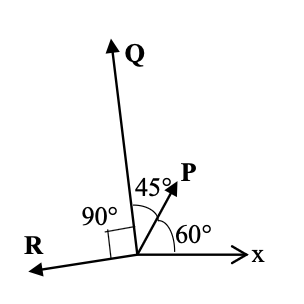
\includegraphics[width=0.5\columnwidth]{GATE/2016/CE/figs/Q39.png} 
    \caption{}
    \label{fig:placeholder}
\end{figure}

\begin{enumerate}
\begin{multicols}{4}
\item 299.90 and $96.0\degree$
\item 368.1 and $94.7\degree$
\item 330.4 and $118.9\degree$
\item 400.1 and $113.5\degree$
\end{multicols}
\end{enumerate}

